\documentclass[a4paper, oneside, openany, dvipsnames, table, 12pt]{article}
\usepackage{../../Template/AFKstyle}
\usepackage{hyperref}
\usepackage{amsmath}
\usepackage{verbatim}
\newcommand{\Titolo}{Verbale interno 2020-06-05}

\newcommand{\Gruppo}{TeamAFK}

\newcommand{\Redattori}{}

\newcommand{\Verificatori}{}

\newcommand{\pathimg}{../../../../Template/img/logoAFK.png}

\newcommand{\Approvatore}{}

\newcommand{\Distribuzione}{Prof. Vardanega Tullio \newline Prof. Cardin Riccardo \newline TeamAFK}

\newcommand{\Uso}{Interno}

\newcommand{\NomeProgetto}{"Predire in Grafana"}

\newcommand{\Mail}{gruppoafk15@gmail.com}

\newcommand{\Versionedoc}{1.0.0}

\newcommand{\DescrizioneDoc}{Riassunto dell'incontro del gruppo \textit{TeamAFK} tenutosi il 2020-06-05.}


\makeindex

%------------------ PER SISTEMARE INDICE TABELLE E FIGURE 
\makeatletter
\renewcommand*\l@figure{\@dottedtocline{1}{1.5em}{3em}}% 3em instead of 2.3em
\let\l@table\l@figure
\makeatother
%------------------

\begin{document}
\copertina{}

%------------------ COLORI TABELLE 
\definecolor{pari}{RGB}{255, 207, 158} %{HTML}{E1F5FE} %azzurrino
\definecolor{dispari}{HTML}{FAFAFA} %bianco/grigetto 

%definizione colori per tabelle (tranne copertina)
\definecolor{redafk}{RGB}{255, 133, 51}
\definecolor{grey2}{RGB}{204, 204, 204}
\definecolor{greyRowafk}{RGB}{234, 234, 234}
\definecolor{lastrowcolor}{RGB}{176, 196, 222} %steel blue %{255,165,0} orange %{RGB}{255, 207, 158}
\rowcolors{2}{pari}{dispari}
\renewcommand{\arraystretch}{1.5}

%------------------

%Didascalia tabelle/immagini (prendono come riferimento la subsection)
\counterwithin{table}{subsection}
\counterwithin{figure}{subsection}
\newpage

%indice, indice figure e indice tabelle
\tableofcontents
\newpage
\listoffigures
\newpage
\listoftables
\newpage

\section{Introduzione}

\subsection{Scopo del documento}
Il seguente documento ha il compito di stabilire le regole che il team di sviluppo intende seguire in ogni attività di progetto, così da omologare il materiale prodotto.
I fornitori intendono adottare un approccio incrementale\glo, affinché lo sviluppo del prodotto si basi su decisioni prese di comune accordo. Perciò ogni componente del team deve far riferimento a questo documento per garantire la coesione e uniformità delle scelte prese.

\subsection{Scopo del prodotto}
Il capitolato {C4}\glo illustra il prodotto da fornire. Tale prodotto consiste in tool di addestramento ed un plugin\glo di Grafana\glo che prenderà il nome \textit{Predire in Grafana}. Entrambi gli applicativi verranno scritti in linguaggio JavaScript\glo. Il primo avrà il compito di produrre un file di estensione JSON\glo basato su dati di addestramento\glo. Il secondo invece si occuperà di leggere il file creato, effettuare previsioni basandosi su di esso e rendere disponibili al sistema i risultati ottenuti, in modo da poterli visualizzare in grafici e dashboard.
\subsection{Glossario}
Per evitare ambiguità nei documenti formali, viene fornito il documento \textit{Glossario\_v2.0.0}, contenente tutti i termini considerati di difficile comprensione. Perciò nella documentazione fornita ogni vocabolo contenuto in \textit{Glossario\_v2.0.0} è contrassegnato dalla lettera \textit{G} a pedice.
\subsection{Riferimenti}
\subsubsection{Riferimenti normativi}
\begin{itemize}
	\item \textbf{Capitolato d'appalto C4 - Predire in Grafana}: \\
	\url{https://www.math.unipd.it/~tullio/IS-1/2019/Progetto/C4.pdf}.	
\end{itemize}
\subsubsection{Riferimenti informativi}
\begin{itemize}
	\item \textbf{Change Management Process}: \\
	\href{https://www.blog-management.it/2018/04/10/change-management-project-management/}{https://www.blog-management.it/change-management-project-management}\\
	\href{https://www.digital4.biz/hr/hr-transformation/digital-transformation-e-change-management-vanno-avanti-di-pari-passo/}{https://www.digital4.biz/hr/hr-transformation/};
	\item \textbf{The three P's of Software Engineering}: \\
	\url{http://dwaynephillips.net/CutterPapers/ppp/ppp.htm}
	\item \textbf{Software Engineering - Ian Sommerville - 10th Edition}
	\item \textbf{Slide L05 del corso Ingegneria del Software - Ciclo di vita del software}: \\
	\url{https://www.math.unipd.it/~tullio/IS-1/2019/Dispense/L05.pdf};
	\item \textbf{Slide L06 del corso Ingegneria del Software - Gestione di Progetto}: \\
	\url{https://www.math.unipd.it/~tullio/IS-1/2019/Dispense/L06.pdf};	
	\item \textbf{Slide L12 del corso Ingegneria del Software - Qualità di Prodotto}: \\
	\url{https://www.math.unipd.it/~tullio/IS-1/2019/Dispense/L12.pdf};
	\item \textbf{Slide L13 del corso Ingegneria del Software - Qualità di Processo}: \\
	\url{https://www.math.unipd.it/~tullio/IS-1/2019/Dispense/L13.pdf};
\end{itemize}
\pagebreak

\section{Architettura del prodotto}

\subsection{Descrizione generale}
Il progetto \textit{Predire in Grafana} prevede la realizzazione di due moduli: un plug-in per la piattaforma Grafana e un tool esterno di supporto, rispettivamente chiamati \textbf{Prediction Plug-in} e \textbf{Prediction Tool}. \\
Il Prediction Tool si occupa di addestrare un algoritmo di \textit{SVM} o \textit{Regressione Lineare} utilizzando un dataset inserito dall'utente, per poi generare un file json contenente le informazioni necessarie per poter effettuare un calcolo di predizione. Questo modulo è stato sviluppato seguendo il pattern \textit{Model-View-ViewModel (MVVM)}.\\
Il Prediction Plug-in invece si occuperà di ricevere in input il json e una volta collegati i predittori, contenuti nel file, ad un flusso dati, permetterà di iniziare ad effettuare i calcoli di previsione. Questo modulo è stato sviluppato seguendo il pattern \textit{Model-View-Controller (MVC)}.\\
Le motivazioni principali che hanno portato alla scelta del design pattern MVVM per il Prediction Tool sono:
\begin{itemize}
	\item per la realizzazione del componente è stato utilizzato \textit{React} e abbiamo ritenuto che questo pattern si accoppiasse bene con la struttura di quest'ultimo.
\end{itemize}
Le motivazioni principali che hanno portato alla scelta del design pattern MVC per il Prediction Plug-in sono:
\begin{itemize}
	\item abbiamo ritenuto che questo pattern si accoppiasse meglio con la struttura dei plug-in di Grafana.
\end{itemize}
Inoltre entrambi i pattern permettono:
\begin{itemize}
	\item di disaccoppiare la parte di \textit{presentation logic} da quella di \textit{business logic};
	\item il riutilizzo di alcune componenti in altri contesti, senza doverli modificare.
\end{itemize}
Di seguito sono mostrati i diagrammi delle attività corrispondenti agli Use Cases descritti nell'\textit{Analisi dei Requisiti}.


\subsubsection{Diagrammi delle attività}
\begin{figure}[H]
\centering
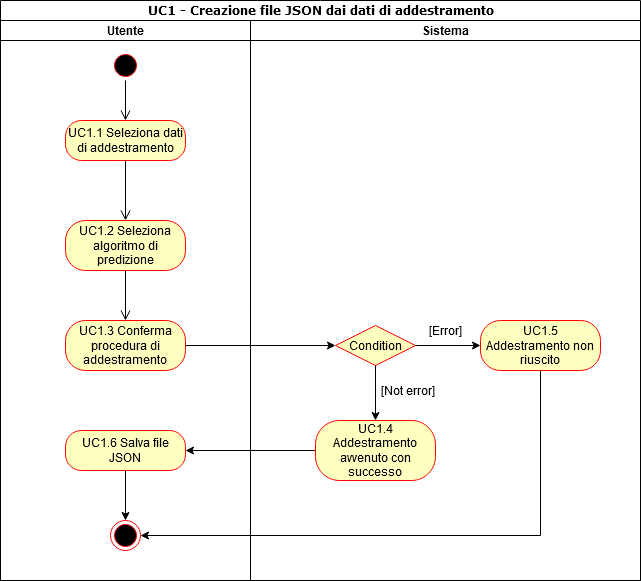
\includegraphics[scale=0.6]{../../Diagrams/Activity_diagrams/uc1.png}
\caption{Diagramma delle attività dello UC1}
\end{figure}
\textbf{Specifica:} lo UC1.5 racchiude i seguenti tipi di errori: 
\begin{itemize}
	\item \textbf{UC7}: Nessun file CSV caricato;
	\item \textbf{UC8}: Nessun algoritmo selezionato;
	\item \textbf{UC9}: File CSV incompatibile.
\end{itemize}
\begin{figure}[H]
\centering
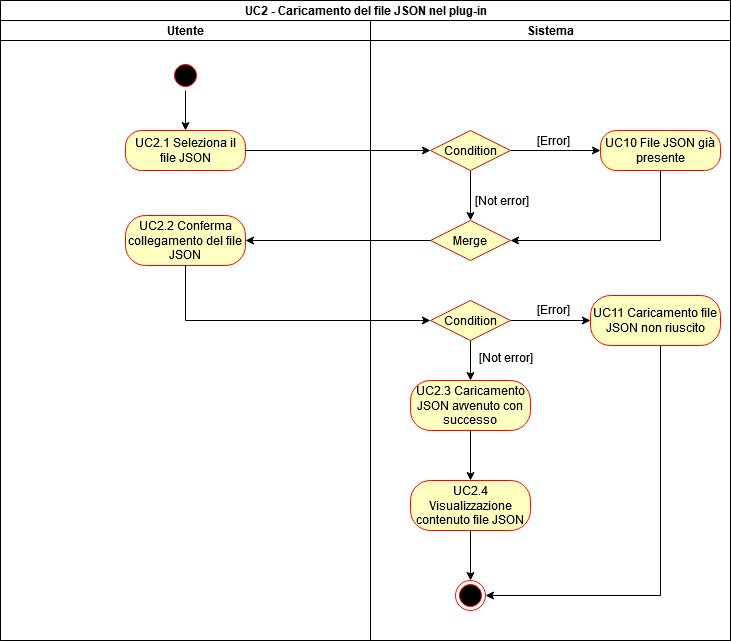
\includegraphics[scale=0.6]{../../Diagrams/Activity_diagrams/uc2.png}
\caption{Diagramma delle attività dello UC2}
\end{figure}
\begin{figure}[H]
\centering
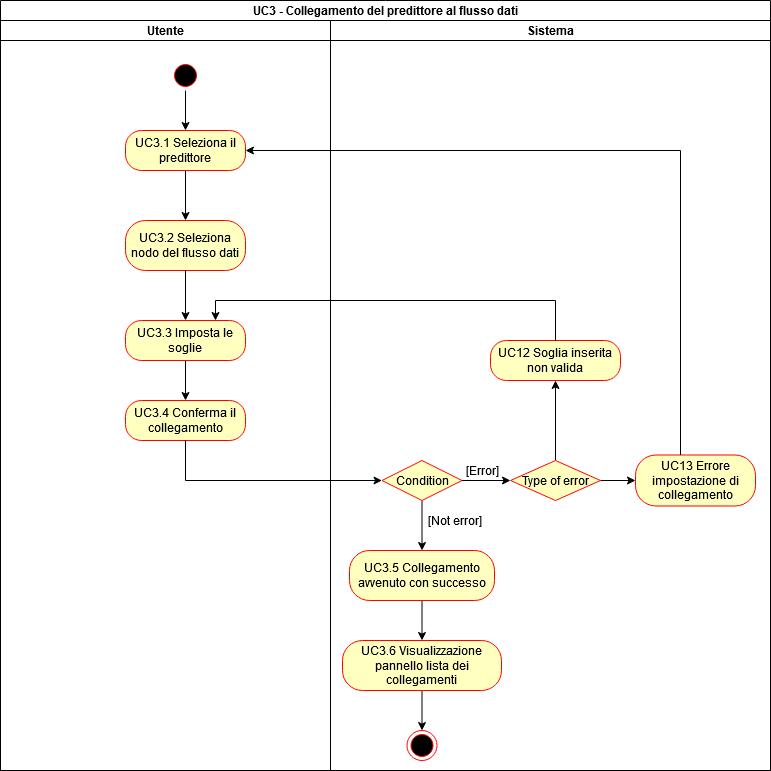
\includegraphics[scale=0.6]{../../Diagrams/Activity_diagrams/uc3.png}
\caption{Diagramma delle attività dello UC3}
\end{figure}
\begin{figure}[H]
\centering
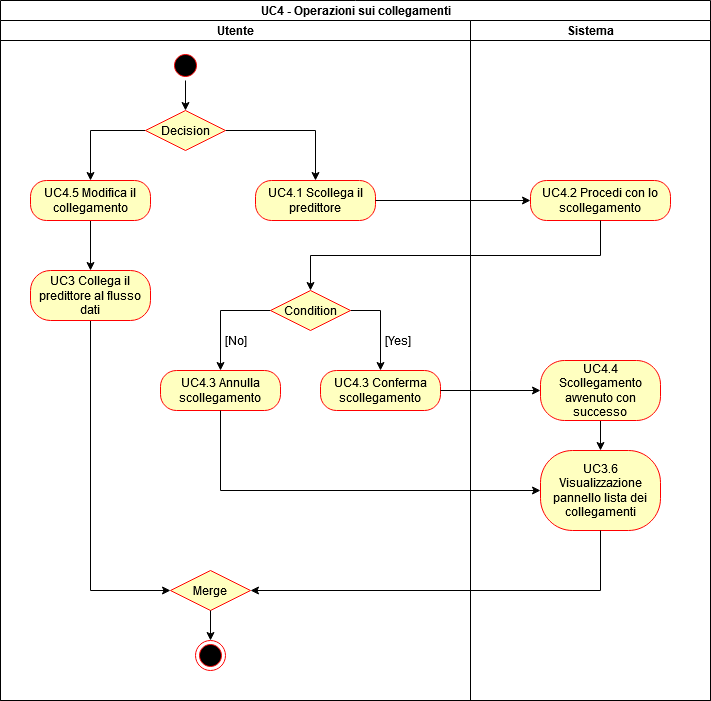
\includegraphics[scale=0.6]{../../Diagrams/Activity_diagrams/uc4.png}
\caption{Diagramma delle attività dello UC4}
\end{figure}
\begin{figure}[H]
\centering
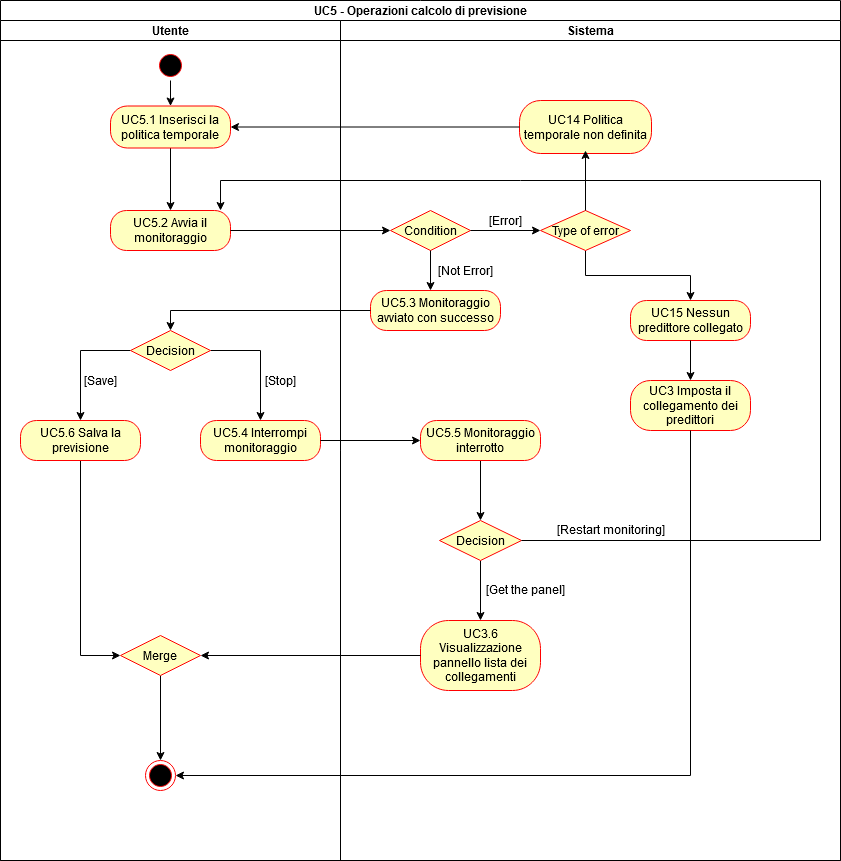
\includegraphics[scale=0.5]{../../Diagrams/Activity_diagrams/uc5.png}
\caption{Diagramma delle attività dello UC5}
\end{figure}
\begin{figure}[H]
\centering
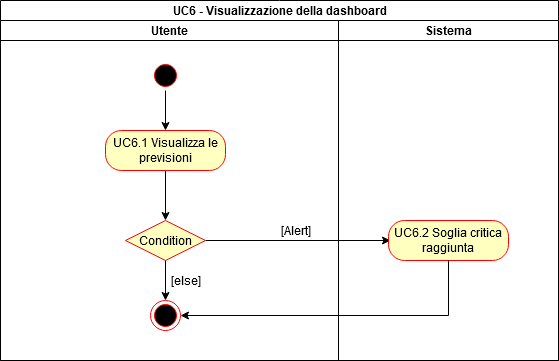
\includegraphics[scale=0.6]{../../Diagrams/Activity_diagrams/uc6.png}
\caption{Diagramma delle attività dello UC6}
\end{figure}

\subsection{Architettura Prediction Tool}

\subsubsection{Descrizione}
L'implemetenazione del tool è stata realizzata utilizzando il design pattern MVVM.
Il passaggio di dati dalle view al model avviene attraverso la modifica di un campo dati \textit{props} immesso dal \textit{ViewModel}.
Attraverso queste \textit{props} il \textit{ViewModel} chiama le funzioni corrette quando l’utente interagisce con la vista.
La divisione tra Business Logic\glo e Presentation Logic è rafforzato da questo utilizzo delle \texttt{props}.
Nel modello viene fornita funzionalità per la gestione degli algoritmi tramite le classi \textit{SVMtrain} e \textit{RLtrain} che verranno utilizzate dal \textit{ViewModel}.


\begin{comment} si trovano un'istanza delle classi SVMtrain e RLtrain in base all'algoritmo scelto, le classi stesse si trovano nel modello e si occupano di rendere polimorfe le funzioni principali, come quelle di addestramento o di recupero del file JSON.
\end{comment}

\subsubsection{Diagrammi dei package}
\begin{figure}[H]
\centering
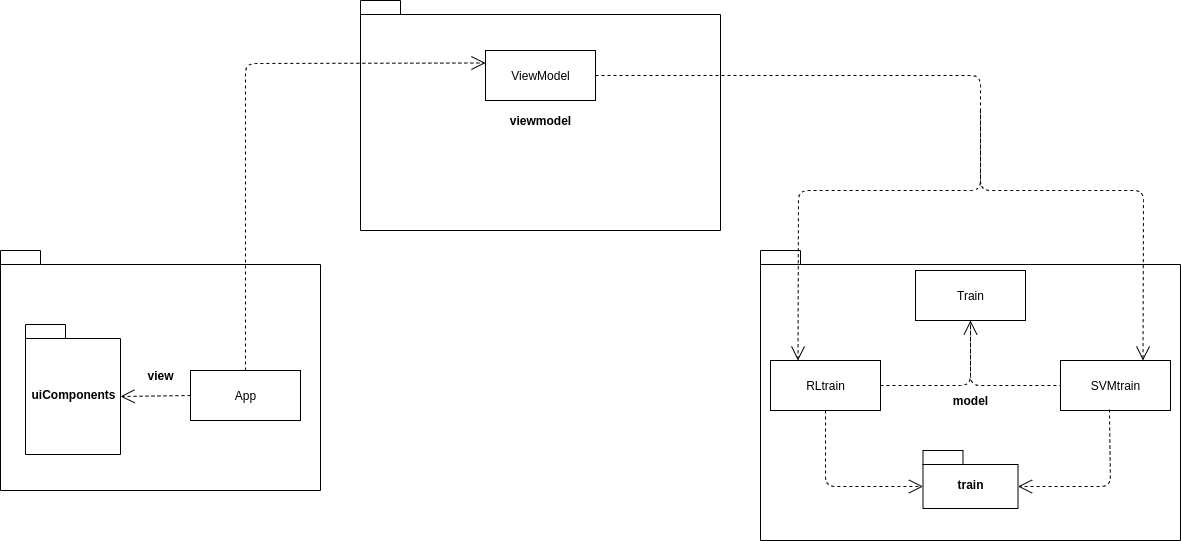
\includegraphics[scale=0.4]{../../Diagrams/Package_diagrams/tool_design_patern.png}
\caption{Diagramma dei package del Prediction Tool}
\end{figure}

\subsubsection{Diagrammi delle classi}
Quello che segue è il diagramma delle classi del Prediction Tool.

\begin{figure}[H]
\centering
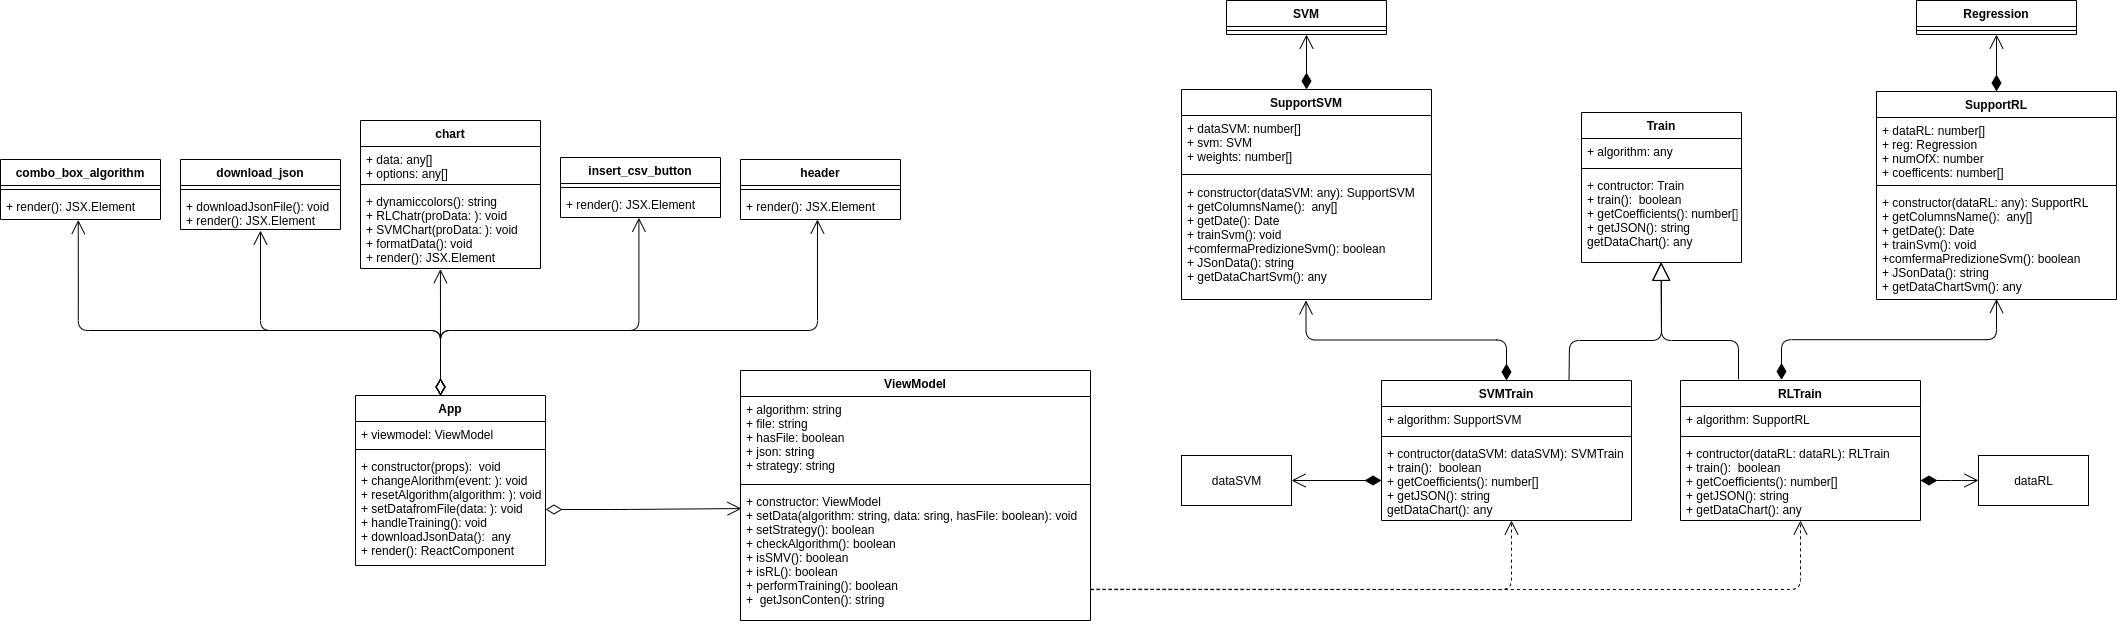
\includegraphics[scale=0.22]{../../Diagrams/Classes_diagrams/tool_all_classes.png}
\caption{Diagramma delle classi del Prediction Tool}
\end{figure}

\begin{comment}
\begin{figure}[H]
\centering
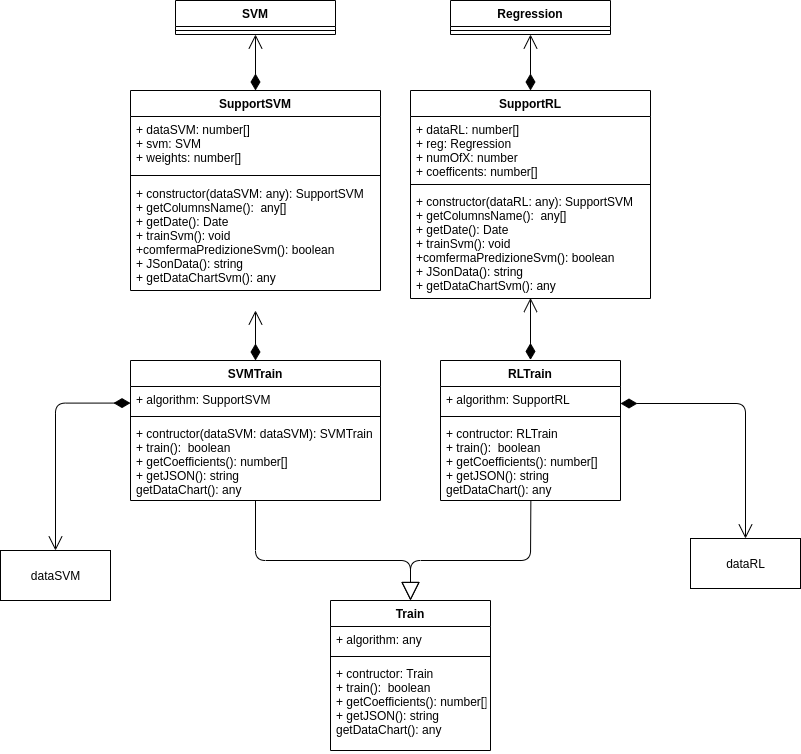
\includegraphics[scale=0.5]{../../Diagrams/Classes_diagrams/tool_model.png}
\caption{Diagramma delle classi del Model del Prediction Tool}
\end{figure}
\pagebreak
\textbf{View}
\begin{figure}[H]
\centering
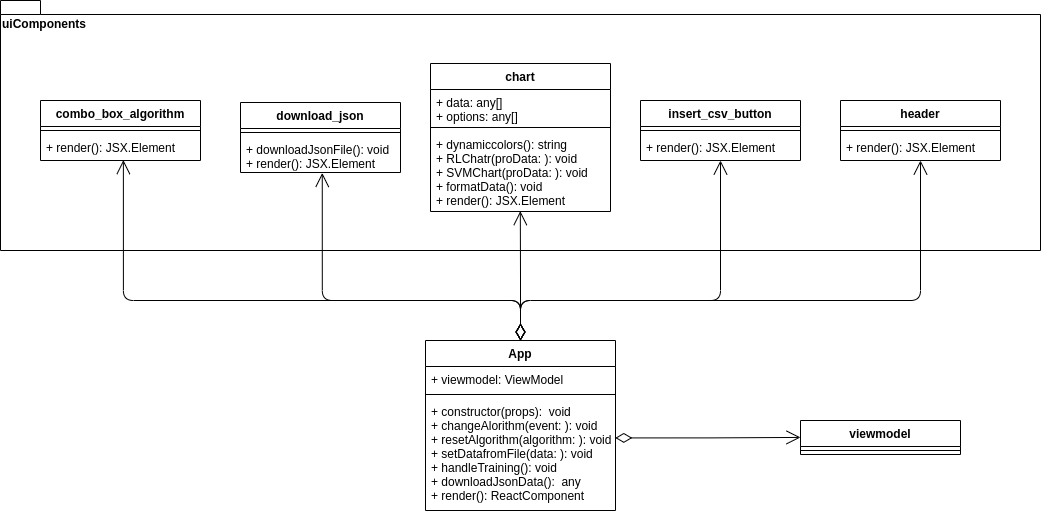
\includegraphics[scale=0.45]{../../Diagrams/Classes_diagrams/tool_view.png}
\caption{Diagramma delle classi della View del Prediction Tool}
\end{figure}

\textbf{ViewModel}
\begin{figure}[H]
\centering
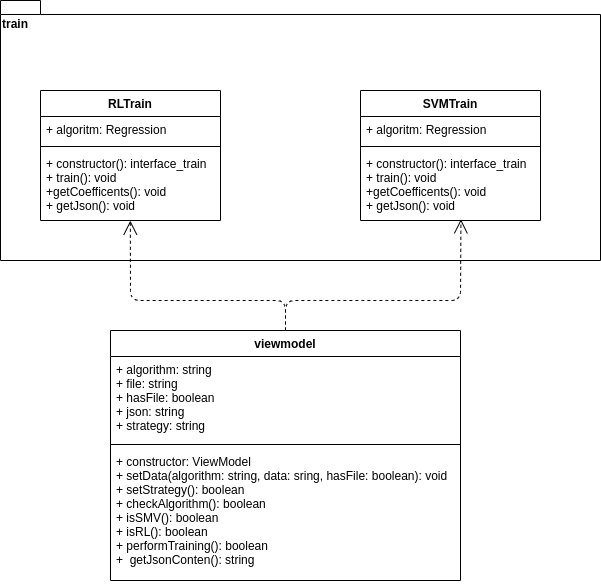
\includegraphics[scale=0.5]{../../Diagrams/Classes_diagrams/tool_modelview.png}
\caption{Diagramma delle classi del ViewModel del Prediction Tool}
\end{figure}
\end{comment}

\subsubsection{Diagrammi di sequenza}
\begin{figure}[H]
\centering
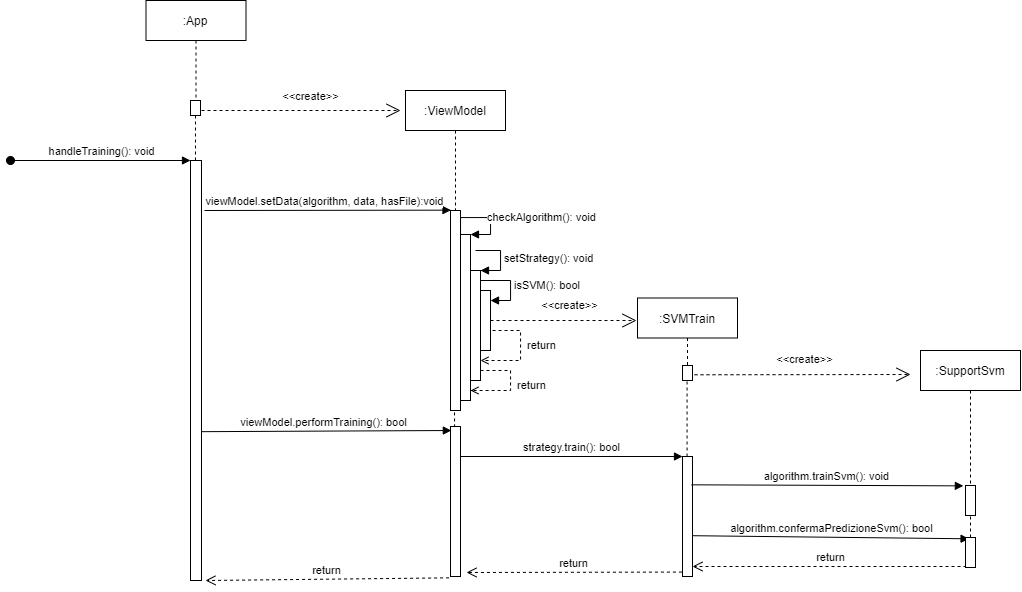
\includegraphics[scale=0.45]{../../Diagrams/Sequence_diagrams/trainSVM.png}
\caption{Diagramma di sequenza del TrainSVM}
\end{figure}

\subsubsection{Design pattern comportamentali utilizzati}
Per quanto riguarda i design pattern comportamentali utilizzati, durante la progettazione delle classi del Prediction Tool ci siamo accorti che alcune classi correlate tra loro (quelle adibite a richiamare le librerie per gli algoritmi di Machine Learning RL e SVM) differivano soltanto per il comportamento effettivo, dato dalla libreria richiamata. I metodi utilizzati dalle due classi erano in effetti più varianti di uno stesso algoritmo (quello di addestramento). Per queste ragioni abbiamo pensato di utilizzare il design pattern \textbf{Strategy}, così da definire una famiglia di algoritmi, incapsularli e renderli interscambiabili tra di loro, a seconda della scelta effettuata dall’utente.
Nel nostro caso abbiamo identificato come \textit{Strategy} l’oggetto contenente un riferimento all'algoritmo di previsione.
Quest'ultimo rappresenta il modello della nostra applicazione, dove è contenuta effettivamente la business logic.

\pagebreak
\subsection{Architettura Prediction Plug-in}

\subsubsection{Descrizione}
In questo modulo, composto da più pannelli all'interno di Grafana, verrà associato il predittore prodotto dal tool esterno al flusso dati monitorato appunto in Grafana. Per questo modulo è stato utilizzato il pattern architetturale \textit{MVC}.
In questa architettura l’Editor e il Panel condividono la variabile \textit{props}, istanziata da Grafana. 
All’importazione del file JSON, il controller si occuperà di: \begin{itemize}
\item leggere il suo contenuto attraverso la funzione \texttt{setJson(file)};
\item salvare una copia dei predittori;
\item applicare l'algoritmo di previsione corretto attraverso il metodo \texttt{setStrategy()};
\item inviare una notifica alla viste di successo caricamento file JSON.
\end{itemize}
\begin{comment}
\textbf{AGGIUNGERE RIGUARDO MODEL E VIEW}
\end{comment}
Per quanto riguarda la comunicazione che avviene tra \textit{View} e \textit{Model} viene gestita dal \textit{Controller}. Questo è stato reso possibile per la presenza in \textit{Editor} di un istanza della classe \textit{Controller}. In questo modo, ad ogni caricamento del file JSON, la vista comunica al \textit{Controller} l'avvenuto caricamento (tramite il metodo \texttt{setJson(file)}) passando come parametro il file appena ricevuto.
Una volta che il \textit{Controller} termina la lettura del file notifica la vista di aggiornarsi (tramite il metodo \texttt{update()}), mostrando le nuove informazioni ottenute dal file.

A seguito di una discussione col proponente, abbiamo deciso di creare una componente Panel come punto di partenza del nostro plug-in, la quale ha il compito di creare una dashboard per permettere all’utente di prendere familiarità con le funzionalità dei vari pannelli.

\subsubsection{Diagrammi dei package}
\begin{figure}[H]
\centering
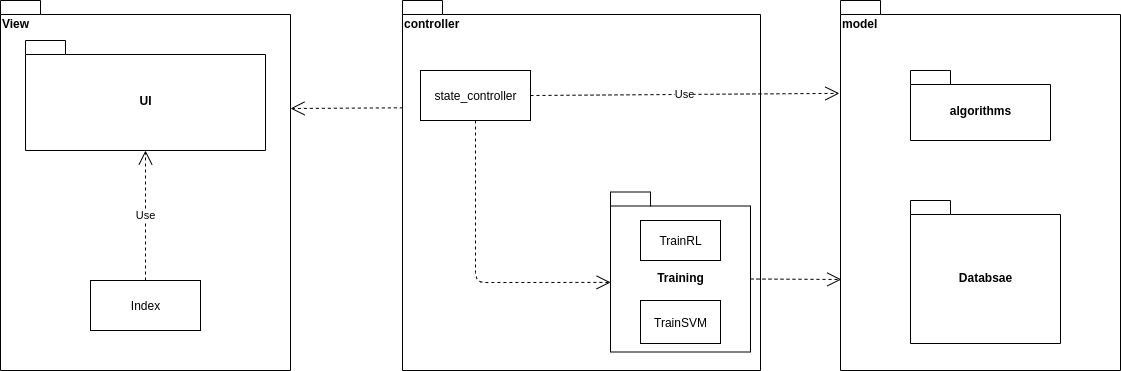
\includegraphics[scale=0.40]{../../Diagrams/Package_diagrams/plugin_design_pattern.png}
\caption{Diagramma dei package del Prediction Plug-in}
\end{figure}

\subsubsection{Diagrammi delle classi}
\textbf{Model}
\begin{figure}[H]
\centering
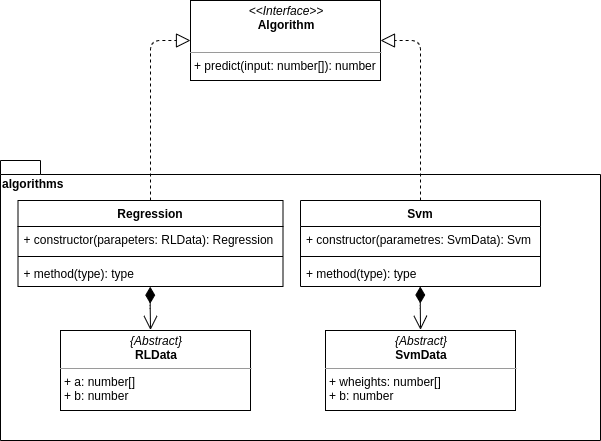
\includegraphics[scale=0.45]{../../Diagrams/Classes_diagrams/plugin_model.png}
\caption{Diagramma delle classi del Model del Prediction Plug-in}
\end{figure}

\textbf{View}
\begin{figure}[H]
\centering
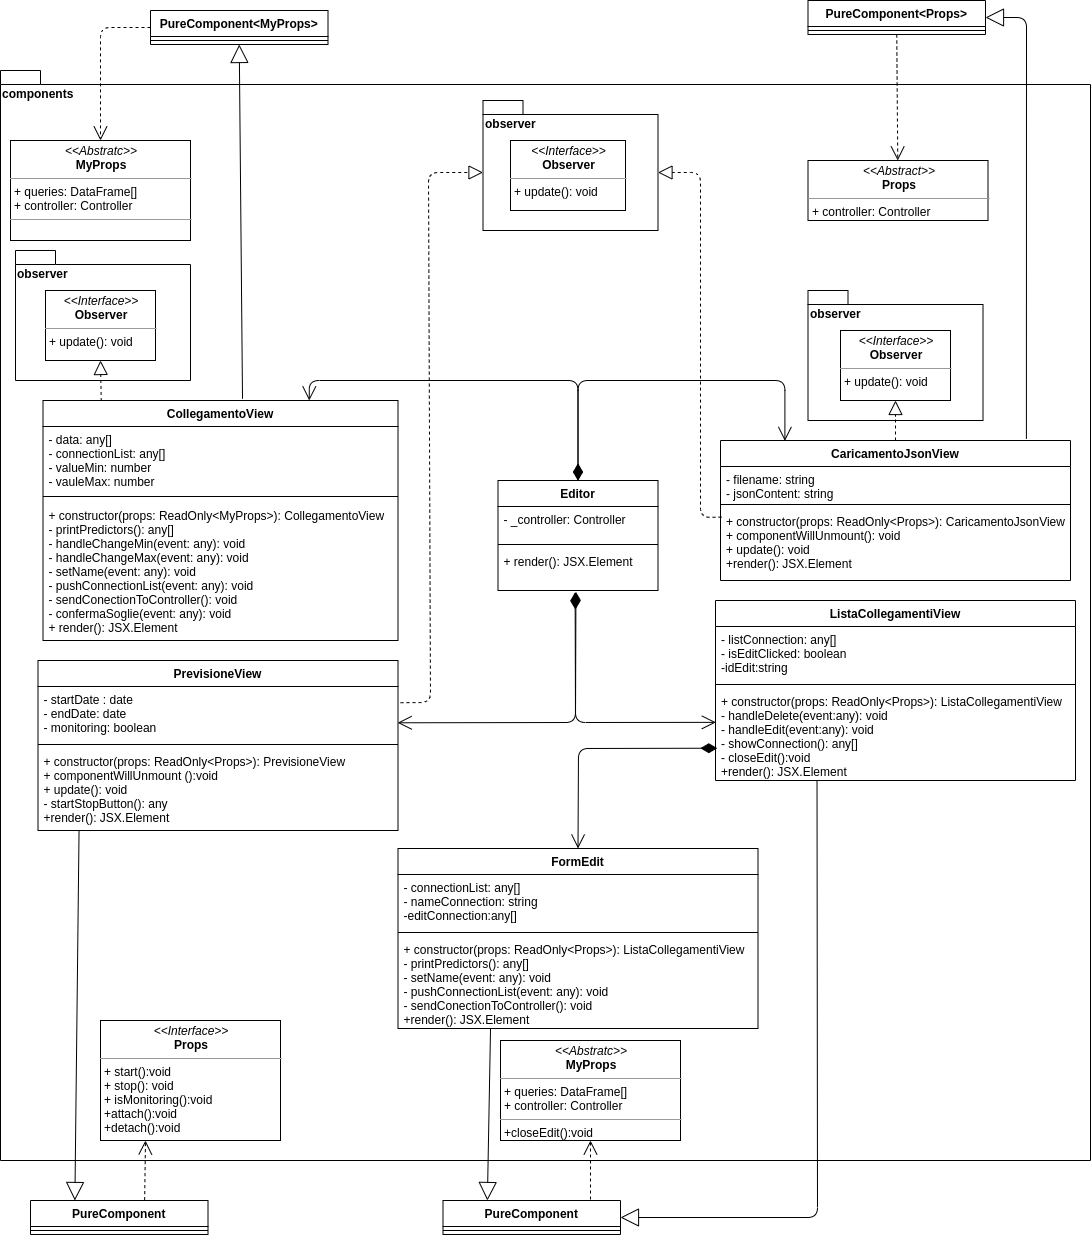
\includegraphics[scale=0.4]{../../Diagrams/Classes_diagrams/plugin_view.png}
\caption{Diagramma delle classi della View del Prediction Plug-in}
\end{figure}

\textbf{Controller}
\begin{figure}[H]
\centering
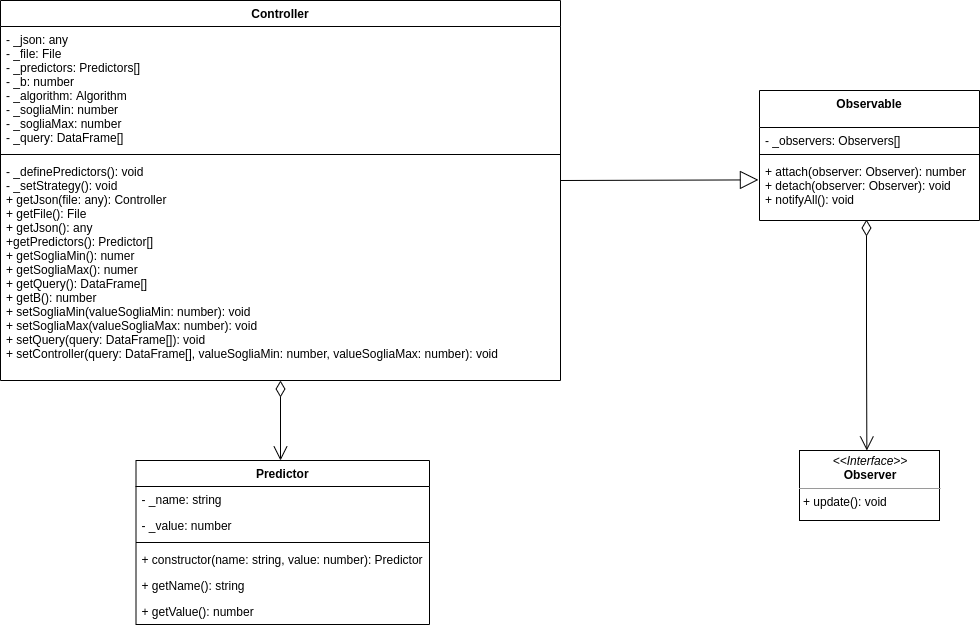
\includegraphics[scale=0.4]{../../Diagrams/Classes_diagrams/plugin_controller.png}
\caption{Diagramma delle classi del Controller del Prediction Plug-in}
\end{figure}

\subsubsection{Diagrammi di sequenza}
\begin{figure}[H]
\centering
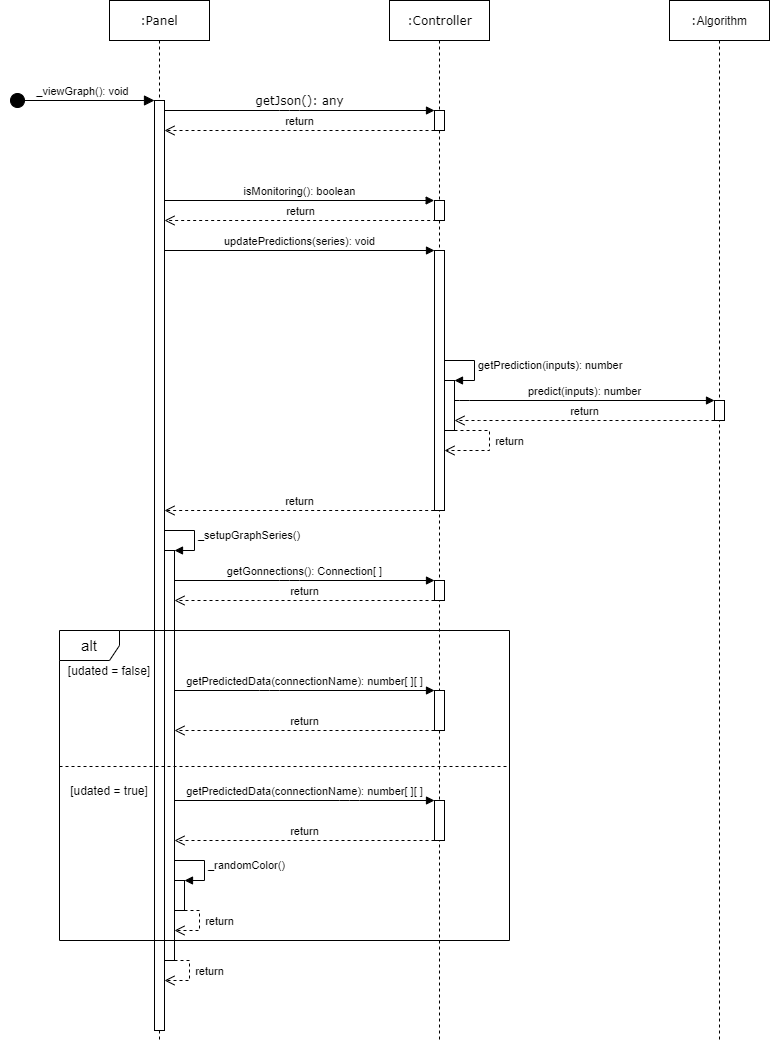
\includegraphics[scale=0.55]{../../Diagrams/Sequence_diagrams/viewGraph.png}
\caption{Diagramma di sequenza del Panel}
\end{figure}

\subsubsection{Design pattern comportamentali utilizzati}
Tra i design pattern che sono stati adottati per l'implementazione del plugin, rientrano l'\textbf{Observer Pattern} e lo \textbf{Strategy Pattern}. \\
L'Observer pattern è stato utilizzato per semplificare la comunicazione tra controller e le componenti della vista che necessitano di essere aggiornate a seguito della modifica dello stato del controler. Infatti nel nostro caso la classe \textit{subject}, ovvero la classe di cui monitorarne lo stato, è la componente controller mentre la componente \textit{Observer}, ovvero tutte le classi che necessitano di essere aggiornate a seguito di un cambiamento dello stato del subject, sono le componenti grafiche utilizzate dalla classe \textit{Editor}. \\
Lo Strategy pattern è stato utilizzato per gli algoritmi di predizione, infatti il controller ha un riferimento all'interfaccia \textit{Algorithm} che espone il metodo \texttt{predict(inputs)}. Nel model sono quindi presenti le classi concrete (\textit{Regression} e \textit{Svm}) che implementano l'algoritmo di predizione e il controller si occupa di istanziare l'algoritmo corretto rispetto quanto letto dal file json.

\pagebreak

\section{Requisiti}
I requisiti sono definiti nelle seguenti tabelle, divise per tipologie.
\begin{comment}
				\begin{itemize}
					\item \textbf{codice identificativo}: è un codice univoco e conforme alla codifica: \\ \\
					\centerline{\textbf{Re[Importanza][Tipologia][Codice]}} \\ \\
					Le voci riportate nella precedente codifica significano: 
					\begin{itemize}
						\item \textbf{Importanza}: la quale può assumere come valori:
						\begin{itemize}
							\item 1: requisito obbligatorio, irrinunciablie;
							\item 2: requisito desiderabile, perciò non obbligatorio ma riconosscibile;
							\item 3: requisito opzionale, ovvero trattabile in un secondo momento o relativamente utile.
						\end{itemize}
						\item \textbf{Tipologia}: la quale può assumere come valori:
						\begin{itemize}
							\item F: funzionale;
							\item P: prestazionale;
							\item Q: qualitativo;
							\item V: vincolo.
						\end{itemize}
						\item \textbf{Codice identificativo}: il quale è un identificatore univoco del requisito, e viene espresso in forma gerarchica padre/figlio.
					\end{itemize}
					\item \textbf{Classificazione}: specifica il peso del requisito facilitando la sua lettura anche se causa ridondanza;
					\item \textbf{Descrizione}: sintesi completa di un requisito;
					\item \textbf{Fonti}: il requisito può avere le seguenti provenienze:
					\begin{itemize}
						\item capitolato;
						\item interno: requisito che gli analisti ritengono di aggiungere in base alle esigenze del team;
						\item caso d'uso: il requisito proviene da uno o più casi d'uso, dei quali è necessario riportare il codice univoco di caso d'uso;
						\item verbale: dopo un chiarimento da parte del proponente è possibile che sorga un requisito non preventivato. E le informazioni su di esso sono riportate e tracciati nei rispettivi verbali.
					\end{itemize}
				\end{itemize} 
				\pagebreak
\end{comment}
\subsection{Requisiti Funzionali}
\begin{longtable}{C{3cm} C{3cm} L{5.5cm} C{3cm}}
\rowcolor{white}\caption{Tabella dei requisiti funzionali} \\
		\rowcolor{redafk}
\textcolor{white}{\textbf{Requisito}} &
\textcolor{white}{\textbf{Classificazione}} &
\textcolor{white}{\textbf{Descrizione}} &
\textcolor{white}{\textbf{Fonti}}  \\
		\endfirsthead
		\rowcolor{white}\caption[]{(continua)} \\
		\rowcolor{redafk}
\textcolor{white}{\textbf{Requisito}} &
\textcolor{white}{\textbf{Classificazione}} &
\textcolor{white}{\textbf{Descrizione}} &
\textcolor{white}{\textbf{Fonti}}  \\
		\endhead
Re1F1 & Obbligatorio & L’utente deve disporre dei dati di addestramento in formato CSV che potrà utilizzare  per creare il file JSON usando l’apposito tool & Capitolato UC1\\
Re1F1.1 & Obbligatorio & All’utente sarà possibile inserire i dati di addestramento cliccando il relativo pulsante &  Interno UC1.1\\
Re1F1.2 & Obbligatorio & All’utente sarà possibile selezionare l’algoritmo con il quale potrà successivamente effettuare i calcoli di previsione dalla relativa ComboBox &  Interno UC1.2\\
Re1F1.3 & Obbligatorio & L’utente potrà confermare le procedure di addestramento impostate cliccando il pulsante di conferma &  Interno UC1.3\\
Re1F1.4 & Obbligatorio & L’utente potrà salvare in locale il file JSON prodotto attraverso il download una volta confermate le procedure di addestramento & Interno UC1.4\\
Re1F2 & Obbligatorio & L’utente potrà caricare il file JSON nel plugin & Capitolato UC2\\
Re1F2.1 & Obbligatorio & L’utente potrà inserire il file JSON cliccando il pulsante di caricamento &  Interno UC2.1\\
Re1F2.2 & Obbligatorio & L’utente potrà confermare il caricamente del file JSON &  Interno UC2.2\\
Re1F3 & Obbligatorio & L’utente avrà la possibilità di collegare il predittore al nodo del flusso dati su cui avverranno i calcoli di previsione &  Capitolato UC3\\
Re1F3.1 & Obbligatorio & L’utente avrà la possibilità di selezionare il predittore dalla lista di predittori contenuti nel file JSON&  Interno UC3.1\\
Re1F3.2 & Obbligatorio & L’utente potrà selezionare una query associata ad un nodo del flusso dati a cui verranno collegati i predittori &  Interno UC3.2\\
Re1F3.3 & Obbligatorio & L’utente potrà impostare delle soglie sui predittori per permettere al sistema di lanciare degli alert &  Capitolato UC3.3\\
Re1F3.4 & Obbligatorio & All’utente sarà possibile confermare il collegamento che verrà aggiunto alla lista dei collegamenti effettuati &  Interno UC3.4\\
Re1F4 & Obbligatorio & L’utente potrà effettuare lo scollegamento di un predittore precedentemente associato &  Interno UC4\\
Re1F5 & Obbligatorio & All’utente sarà possibile apportare delle modifiche ad un collegamento precedentemente effettuato & Capitolato UC5\\
Re1F6 & Obbligatorio & L’utente potrà effettuare operazioni di calcolo di previsione tramite l'avvio del monitoraggio sui collegamenti tra predittori e nodo del flusso dati &  Capitolato UC6\\
Re1F6.1 & Obbligatorio & L’utente potrà inserire la politica temporale per il ricalcolo di previsione &  Interno UC6.1\\
Re1F6.2 & Obbligatorio & L’utente avrà la possibilità di avviare il monitoraggio cliccando il relativo pulsante &  Interno UC6.2\\
Re1F6.3 & Obbligatorio & All’utente sarà offerta la possibilità di effettuare il salvataggio delle previsioni all'interno del DB &  Verbale VI\_2020-03-31\\
Re1F7 & Obbligatorio & L’utente potrà interrompere il monitoraggio cliccando il relativo pulsante& Interno UC7\\
Re1F8 & Obbligatorio & L’utente potrà visualizzare le previsioni attraverso grafici all'interno della dashboard &  Capitolato UC8\\
Re1F9 & Obbligatorio & All’utente sarà mostrato il messaggio di errore file CSV incompatibile con l'algoritmo selezionato &  Interno UC1.1\\
Re1F10 & Obbligatorio & All’utente sarà mostrato un messaggio di avviso il quale segnalerà che il caricamento del file JSON è già avvenuto &  Interno UC2.1\\
Re1F11 & Obbligatorio & L’utente vedrà un messaggio che segnalerà l’errato caricamento del file JSON dovuto a una struttura incompatibile &  Interno UC2.2\\
Re1F12 & Obbligatorio & All’utente verrà segnalato di aver selezionato una soglia non valida attraverso un messaggio di errore &  Interno
UC3.3\\
Re1F13 & Obbligatorio & 
L’utente riceverà un messaggio d’errore segnalante l’errata impostazione di un collegamento & Interno UC3.4\\
Re1F14 & Obbligatorio & L’utente vedrà una notifica di errore avvisandolo di non aver definito una politica temporale &  Interno UC6.2\\
Re1F15 & Obbligatorio & L’utente verrà notificato attraverso un messaggio di errore che lo avviserà di non aver collegato alcun predittore  &  Interno
UC6.2\\
Re1F16 & Obbligatorio & L’utente verrà notificato attraverso un messaggio di addestramento riuscito con successo  & Interno UC1.3\\
Re1F17 & Obbligatorio & L’utente riceverà un messaggio che confermerà che il caricamento del file JSON è avvenuto con successo &  Interno UC2.2\\
Re1F18 & Obbligatorio & L’utente verrà notificato attraverso un messaggio del collegamento avvenuto con successo &  Interno
UC3.4\\
Re1F19 & Obbligatorio & L’utente visualizzerà il pannello con la lista dei collegamenti & Interno UC3.4\\
Re1F20 & Obbligatorio & L’utente verrà notificato con un messaggio che è possibile procedere con lo scollegamento &  Interno UC4\\
Re1F21 & Obbligatorio & L’utente riceverà un messaggio che lo notificherà di aver avviato il monitoraggio con successo  & Interno UC6.2\\
Re1F22 & Obbligatorio & L’utente verrà notificato attraverso un messaggio di aver interrotto il monitoraggio &  Interno UC7\\
Re1F23 & Obbligatorio & L’utente visualizzerà un messaggio che i dati di previsione verranno salvati all’interno del database & Interno UC6.3\\
Re3F24 & Opzionale & L’utente riceverà un messaggio di alert che segnalerà il raggiungimento di soglia critica & Capitolato UC3.3\\
\end{longtable}

%%%%%%%%%%%%%%%%%%%%%%%%%%%%%%%%%

\pagebreak
 	\subsection{Requisiti di Qualità}

\begin{longtable}{C{3cm} C{3cm} L{5.5cm} C{3cm}}
\rowcolor{white}\caption{Tabella dei requisiti di qualità} \\
		\rowcolor{redafk}
\textcolor{white}{\textbf{Requisito}} &
\textcolor{white}{\textbf{Classificazione}} &
\textcolor{white}{\textbf{Descrizione}} &
\textcolor{white}{\textbf{Fonti}}  \\
		\endfirsthead
		\rowcolor{white}\caption[]{(continua)} \\
		\rowcolor{redafk}
\textcolor{white}{\textbf{Requisito}} &
\textcolor{white}{\textbf{Classificazione}} &
\textcolor{white}{\textbf{Descrizione}} &
\textcolor{white}{\textbf{Fonti}}  \\
		\endhead
Re1Q1 & Obbligatorio & La codifica e la progettazione devono rispettare le norme definite nel documento \emph{Piano\_di\_Qualifica v1.0.0} & Interno\\
Re1Q2 & Obbligatorio & E’ necessario rendere disponibile un manuale utente per l’utilizzo del prodotto &  Capitolato\\
Re1Q2.1 & Obbligatorio & Il manuale utente deve essere disponibile in lingua inglese  & Interno\\
Re2Q2.2 & Desiderabile & Il manuale utente deve essere disponibile in lingua italiana &  Interno\\
Re1Q3 & Obbligatorio & E’ necessario rendere disponibile un manuale per la manutenzione ed estensione del prodotto & Capitolato\\
Re1Q4 & Obbligatorio & Il prodotto deve essere sviluppato in modo concorde a quanto stabilito nelle \emph{Norme\_di\_Progetto\_v2.0.0} & Capitolato\\
Re2Q5 & Desiderabile & Il codice sorgente deve essere disponibile in una repository pubblica su GitHub\glo o su altre piattaforme & Capitolato\\
Re2Q6 & Desiderabile & Il plug-in deve essere caricato nella sezione \href{https:// grafana.com/plugins}{Grafana Labs Plugins} & Interno\\
Re2Q7 & Obbligatorio & Il codice sorgente del plug-in deve essere open source\glo & Capitolato\\
\end{longtable}

%%%%%%%%%%%%%%%%%%%%%%%%%%
\pagebreak
	\subsection{Requisiti di Vincolo}

\begin{longtable}{C{3cm} C{3cm} L{5.5cm} C{3cm}}
\rowcolor{white}\caption{Tabella dei requisiti di vincolo} \\
		\rowcolor{redafk}
\textcolor{white}{\textbf{Requisito}} &
\textcolor{white}{\textbf{Classificazione}} &
\textcolor{white}{\textbf{Descrizione}} &
\textcolor{white}{\textbf{Fonti}}  \\
		\endfirsthead
		\rowcolor{white}\caption[]{(continua)} \\
		\rowcolor{redafk}
\textcolor{white}{\textbf{Requisito}} &
\textcolor{white}{\textbf{Classificazione}} &
\textcolor{white}{\textbf{Descrizione}} &
\textcolor{white}{\textbf{Fonti}}  \\
		\endhead
Re1V1 & Obbligatorio & Il Sistema deve essere supportato su browser differenti & Supporto al linguaggio ECMAScript6\\
Re1V1.1 & Obbligatorio & Il Sistema deve essere supportato sul browser Microsoft Edge dalla versione 14 & Supporto al linguaggio ECMAScript6\\
Re1V1.2 & Obbligatorio & Il Sistema deve essere supportato sul browser Chrome dalla versione 58 &  Supporto al linguaggio ECMAScript6\\
Re1V1.3 & Obblifgatorio & Il Sistema deve essere supportato sul browser Firefox dalla versione 54 &   Supporto al linguaggio ECMAScript6\\
Re1V1.4 & Obbligatorio & Il Sistema deve essere supportato sul browser Safari dalla versione 10 &  Supporto al linguaggio ECMAScript6\\
Re1V2 & Obbligatorio & Il file contenente i dati di addestramento deve essere in formato CSV &  Verbale VI\_2020-03-31\\
Re1V3 & Obbligatorio & L’applicazione deve essere sviluppata utilizzando JavaScript 6 (ES6) & Capitolato\\
Re1V4 & Desiderabile & Il tool di addestramento deve essere sviluppato utilizzando il framework React\glo & Interno\\
Re1V5 & Obbligatorio & Lo sviluppo dell’interfaccia del plug-in è realizzato attraverso l’uso di tecnologie web\glo & Interno\\
\end{longtable}

%%%%%%%%%%%%%%%%%%%%%%%%%%%%%%
\pagebreak
	\subsection{Requisiti prestazionali}{
Non sono stati individuati requisiti prestazionali in quanto il progetto sarà costituito da un tool di addestramento e un plug-in. Come database di supporto verrà utilizzato InfluxDB che renderà più efficiente la gestione e la reperibilità dei dati temporali. Essendo l’esecuzione del plug-in affidata alla piattaforma “Grafana”  le prestazioni dipenderanno dalla condizione dei server della piattaforma stessa.}

%%%%%%%%%%%%%%%%%%%%%%%%%%%%%%

\pagebreak
	\subsection{Tracciamento}
		
		\subsubsection{Fonte - Requisiti}

\begin{longtable}{C{3cm} C{3cm} L{5.5cm} C{3cm}}
\rowcolor{white}\caption{Tabella di tracciamento fonte-requisiti} \\
		\rowcolor{redafk}
\textcolor{white}{\textbf{Fonte}} &
\textcolor{white}{\textbf{Requisiti}} \\
		\endfirsthead
		\rowcolor{white}\caption[]{(continua)} \\
		\rowcolor{redafk}
\textcolor{white}{\textbf{Fonte}} &
\textcolor{white}{\textbf{Requisiti}} \\
		\endhead
Capitolato & Re1F1\newline Re1F2 \newline Re1F3 \newline Re1F3.3 \newline Re1F5 \newline Re1F6 \newline Re1F8 \newline Re3F24\newline Re1Q2\newline Re1Q3\newline Re1Q4\newline Re1Q5\newline Re1V3\\
Interno & Re1F1.1\newline Re1F1.2\newline Re1F1.3\newline Re1F1.4\newline Re1F2.1\newline Re1F2.2\newline Re1F3.1\newline Re1F3.2\newline Re1F3.4\newline Re1F4\newline Re1F6.1\newline  Re1F6.2\newline Re1F7\newline Re1F9\newline Re1F10\newline Re1F11\newline Re1F12\newline  Re1F13\newline  Re1F14\newline  Re1F15\\
Interno & Re1F16 \newline Re1F17\newline  Re1F18\newline Re1F19\newline  Re1F20\newline  Re1F21\newline  Re1F22\newline  Re1F23\newline  Re1Q1\newline  Re1Q2.1\newline  Re2Q2.2\newline  Re2Q6\newline  Re1V4
\newline  Re1V6\\
UC1 & Re1F1\\
UC1.1 & Re1F1.1\newline Re1F9\\
UC1.2 & Re1F1.2\\
UC1.3 & Re1F1.3\newline Re1F16\\
UC1.4 & Re1F1.4\\
UC2 & Re1F2\\
UC2.1 & Re1F2.1\newline Re1F10\\
UC2.2 & Re1F2.2\newline Re1F11\newline Re1F17\\
UC3 & Re1F3\\
UC3.1 & Re1F3.1\\
UC3.2 & Re1F3.2\\
UC3.3 & Re1F3.3\newline  Re1F12\newline Re1F24\\
UC3.4 & Re1F3.4\newline Re1F13\newline Re1F18\newline Re1F19\\
UC4 & Re1F4\newline Re1F20\\
UC5 & Re1F5\\
UC6 & Re1F6\\
UC6.1 & Re1F6.1\\
UC6.2 & Re1F6.2\newline Re1F14\newline Re1F15\newline Re1F21\\
UC6.3 & Re1F23\\
UC7 & Re1F7\newline Re1F22\\
UC8 & Re1F8\\
Verbale VI\_2020-03-31 & Re1F6.3\newline Re1V2\\
Supporto al linguaggio ECMAScript6 & Re1V1\newline Re1V1.1\newline Re1V1.2\newline Re1V1.3\newline Re1V1.4\\
\end{longtable}	
\pagebreak
		\subsubsection{Requisito - Fonti}

\begin{longtable}{C{3cm} C{3cm} L{5.5cm} C{3cm}}
\rowcolor{white}\caption{Tabella di tracciamento requisito-fonti} \\
		\rowcolor{redafk}
\textcolor{white}{\textbf{Requisito}} &
\textcolor{white}{\textbf{Fonte}} \\
		\endfirsthead
		\rowcolor{white}\caption[]{(continua)} \\
		\rowcolor{redafk}
\textcolor{white}{\textbf{Requisito}} &
\textcolor{white}{\textbf{Fonte}} \\
		\endhead
Re1F1 & Capitolato\newline UC1\\
Re1F1.1 & Interno\newline UC1.1\\
Re1F1.2 & Interno\newline UC1.2\\
Re1F1.3 & Interno\newline UC1.3\\
Re1F1.4 & Interno\newline UC1.4\\
Re1F2 & Capitolato\newline UC2\\
Re1F2.1 & Interno\newline UC2.1\\
Re1F2.2 & Interno\newline UC2.2\\
Re1F3 & Capitolato\newline UC3\\
Re1F3.1 & Interno\newline UC3.1\\
Re1F3.2 & Interno\newline UC3.2\\
Re1F3.3 & Capitolato\newline UC3.3\\
Re1F3.4 & Interno\newline UC3.4\\
Re1F4 & Interno\newline UC4\\
Re1F5 & Capitolato\newline UC5\\
Re1F6 & Capitolato\newline UC6\\
Re1F6.1 & Interno\newline UC6.1\\
Re1F6.2 & Interno\newline UC6.2\\
Re1F6.3 & Verbale VI\_2020-03-31\\
Re1F7 & Interno\newline UC7\\
Re1F8 & Capitolato\newline UC8\\
Re1F9 & Interno\newline UC1.1\\
Re1F10 & Interno\newline UC2.1\\
Re1F11 & Interno\newline UC2.2\\
Re1F12 & Interno\newline UC3.3\\
Re1F13 & Interno\newline UC3.4\\
Re1F14 & Interno\newline UC6.2\\
Re1F15 & Interno\newline UC6.2\\
Re1F16 & Interno\newline UC1.3\\
Re1F17 & Interno\newline UC2.2\\
Re1F18 & Interno\newline UC3.4\\
Re1F19 & Interno\newline UC3.4\\
Re1F20 & Interno\newline UC4\\
Re1F21 & Interno\newline UC6.2\\
Re1F22 & Interno\newline UC7\\
Re1F23 & Interno\newline UC6.3\\
Re3F24 & Capitolato\newline UC3.3\\
Re1Q1 & Interno\\
Re1Q2 & Capitolato\\
Re1Q2.1 & Interno\\
Re2Q2.2 & Interno\\
Re1Q3 & Capitolato\\
Re1Q4 & Capitolato\\
Re2Q5 & Capitolato\\
Re2Q6 & Interno\\
Re2Q7 & Capitolato\\
Re1V1 & Supporto al linguaggio ECMAScript6\\
Re1V1.1 & Supporto al linguaggio ECMAScript6\\
Re1V1.2 & Supporto al linguaggio ECMAScript6\\
Re1V1.3 & Supporto al linguaggio ECMAScript6\\
Re1V1.4 & Supporto al linguaggio ECMAScript6\\
Re1V2 & Verbale VI\_2020-03-31\\
Re1V3 & Capitolato\\
Re1V4 & Interno\\
Re1V5 & Capitolato\\
\end{longtable}
	
%%%%%%%%%%%%%%%%%%%%%%%%%%%%%%

	\subsection{Considerazioni}
Nel caso in cui le attività pianificate dovessero terminare in anticipo e dovessero avanzare ore di lavoro, i requisiti potrebbero subire alcune modifiche o aggiunte, per permettere la revisione delle voci presenti o delle migliorie. Dunque eventuali aggiornamenti sono lasciati a momenti
futuri.



\pagebreak

\end{document}